\documentclass{beamer}

\usecolortheme[light]{solarized}

\beamertemplatenavigationsymbolsempty

\usepackage{graphicx}
\usepackage{hyperref}
\usepackage{colortbl, xcolor}
\usepackage{booktabs}

\usepackage{tikz}
\usetikzlibrary{calc}

\title{My experiences of being an SSI fellow}
\author{@drvinceknight}
\date{2016-09-09}

\begin{document}

\frame{\titlepage}

\frame{
    \frametitle{What I do.}
\begin{center}

    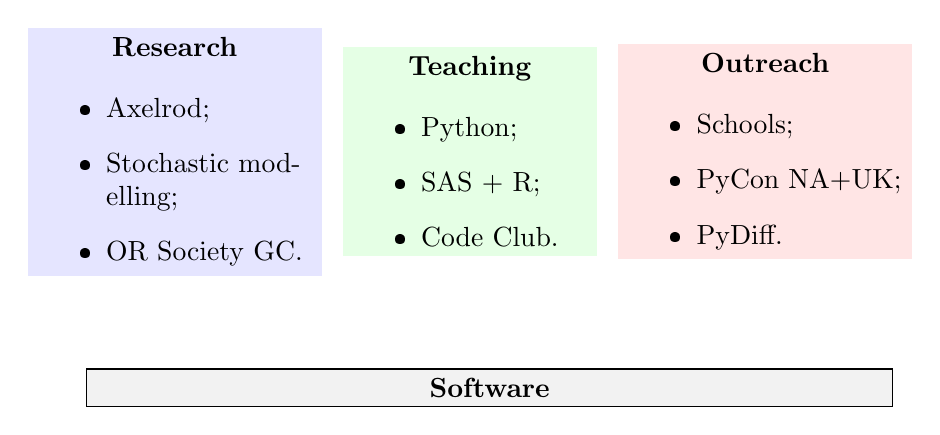
\begin{tikzpicture}
        \node (Research) at (0, 0) [fill=blue!10, text width=3.5cm, align=center]
{\textbf{Research}\\
\begin{itemize}
\item Axelrod;
\item Stochastic modelling;
\item OR Society GC.
\end{itemize}
};
        \node (Teaching) at ($ (Research) + (3.75,0)$) [fill=green!10, text width=3cm, align=center]
{\textbf{Teaching}\\
\begin{itemize}
\item Python;
\item SAS + R;
\item Code Club.
\end{itemize}
};
        \node (Outreach) at ($ (Teaching) + (3.75, 0)$) [fill=red!10, align=center, text width=3.5cm, align=center]
{\textbf{Outreach}\\
\begin{itemize}
\item Schools;
\item PyCon NA+UK;
\item PyDiff.
\end{itemize}
};

\pause

\node at ($(Research) + (4, -3)$) [draw, fill=gray!10, text width=10cm, align=center] {\textbf{Software}};

    \end{tikzpicture}

\end{center}
}

\begin{frame}
    \frametitle{Why did I apply.}
    \pause
    \begin{itemize}
        \item Development.
            \pause
        \item Recognition.
            \pause
        \item People.
    \end{itemize}
\end{frame}

\begin{frame}
    \frametitle{Commitment.}
    \only<2>{
    \begin{center}
        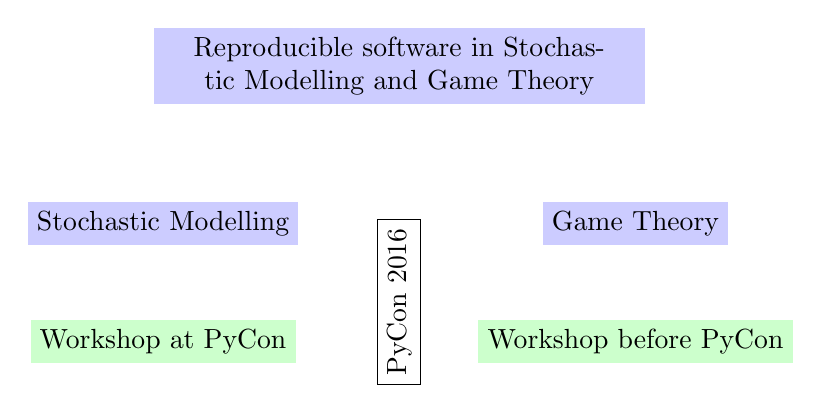
\begin{tikzpicture}
            \node (title) at (0,0) [fill=blue!20, text width = 6cm, align=center]
            {Reproducible software in Stochastic Modelling and Game Theory};
            \node (StochasticModelling) at ($(title) + (-3, -2)$) [fill=blue!20]
            {Stochastic Modelling};

            \node (PyCon) at ($(StochasticModelling) + (0, -1.5)$) [fill=green!20]
            {Workshop at PyCon};

            %-----------------

            \node (GameTheory) at ($(title) + (3, -2)$) [fill=blue!20] {Game Theory};

            \node (gt) at ($(GameTheory) + (0, -1.5)$) [fill=green!20]
            {Workshop before PyCon};

            {Game Theory};

            \pause

            \node (PyConuk) at (0, -3) [rotate=90, draw] {PyCon 2016};
        \end{tikzpicture}
    \end{center}
}
    \only<3>{
        \begin{center}
            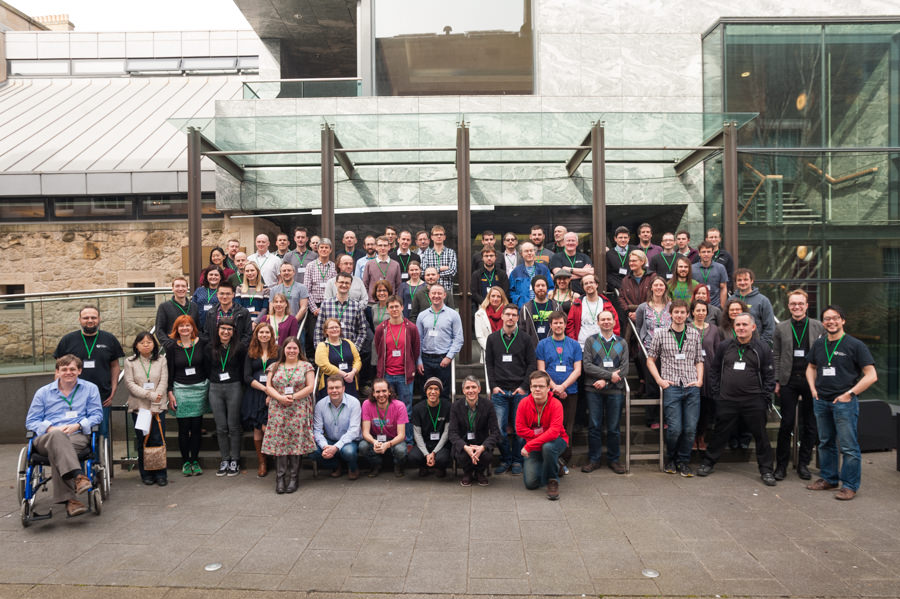
\includegraphics[width=.8\textwidth]{img/cw16-group-photo.jpg}
        \end{center}
    }
\end{frame}

\begin{frame}
    \frametitle{Benefits.}
    \begin{center}
        
\includegraphics[width=.95\textwidth]{img/slack-qstn.png}
    \end{center}
\end{frame}

\end{document}
